\section{Additional plots}\label{sec:appendix_figs}
\begin{figure}[H]
  \centering
  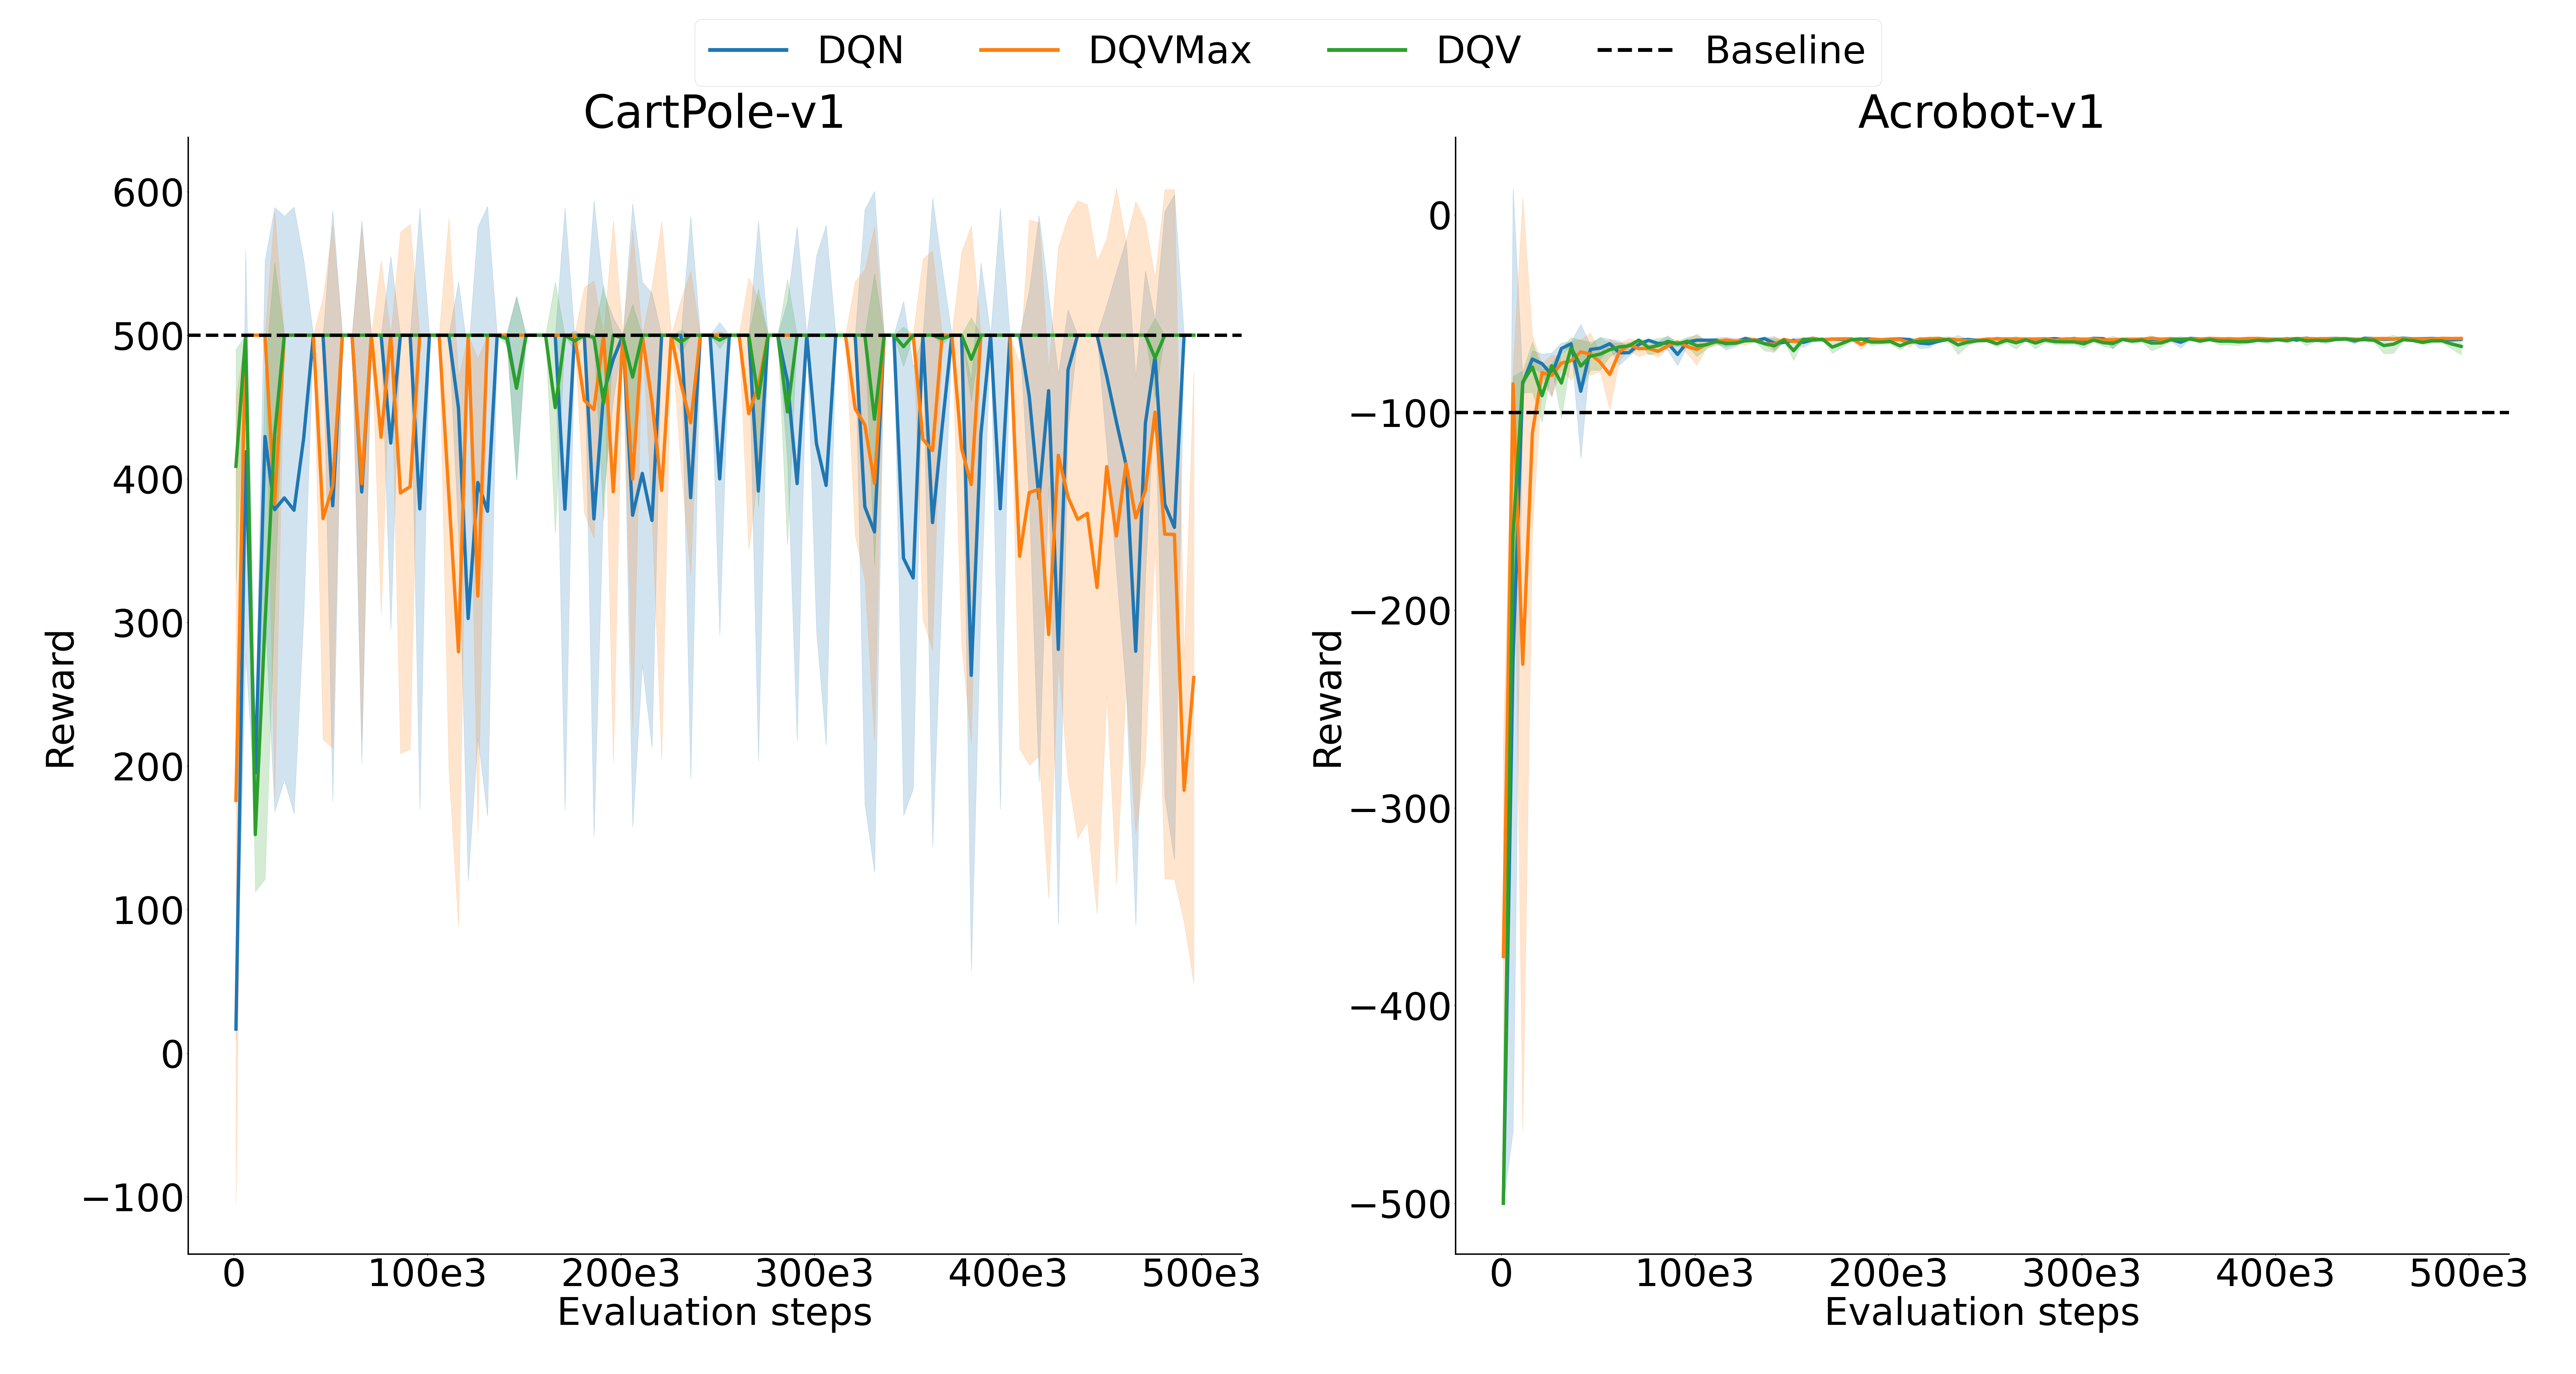
\includegraphics[width=.5\textwidth]{img/dshift_plots_rwd.png}
  \caption{Standard agents reward signal}\label{fig:dshift_rwd}
\end{figure}

\begin{figure}[H]
  \centering
  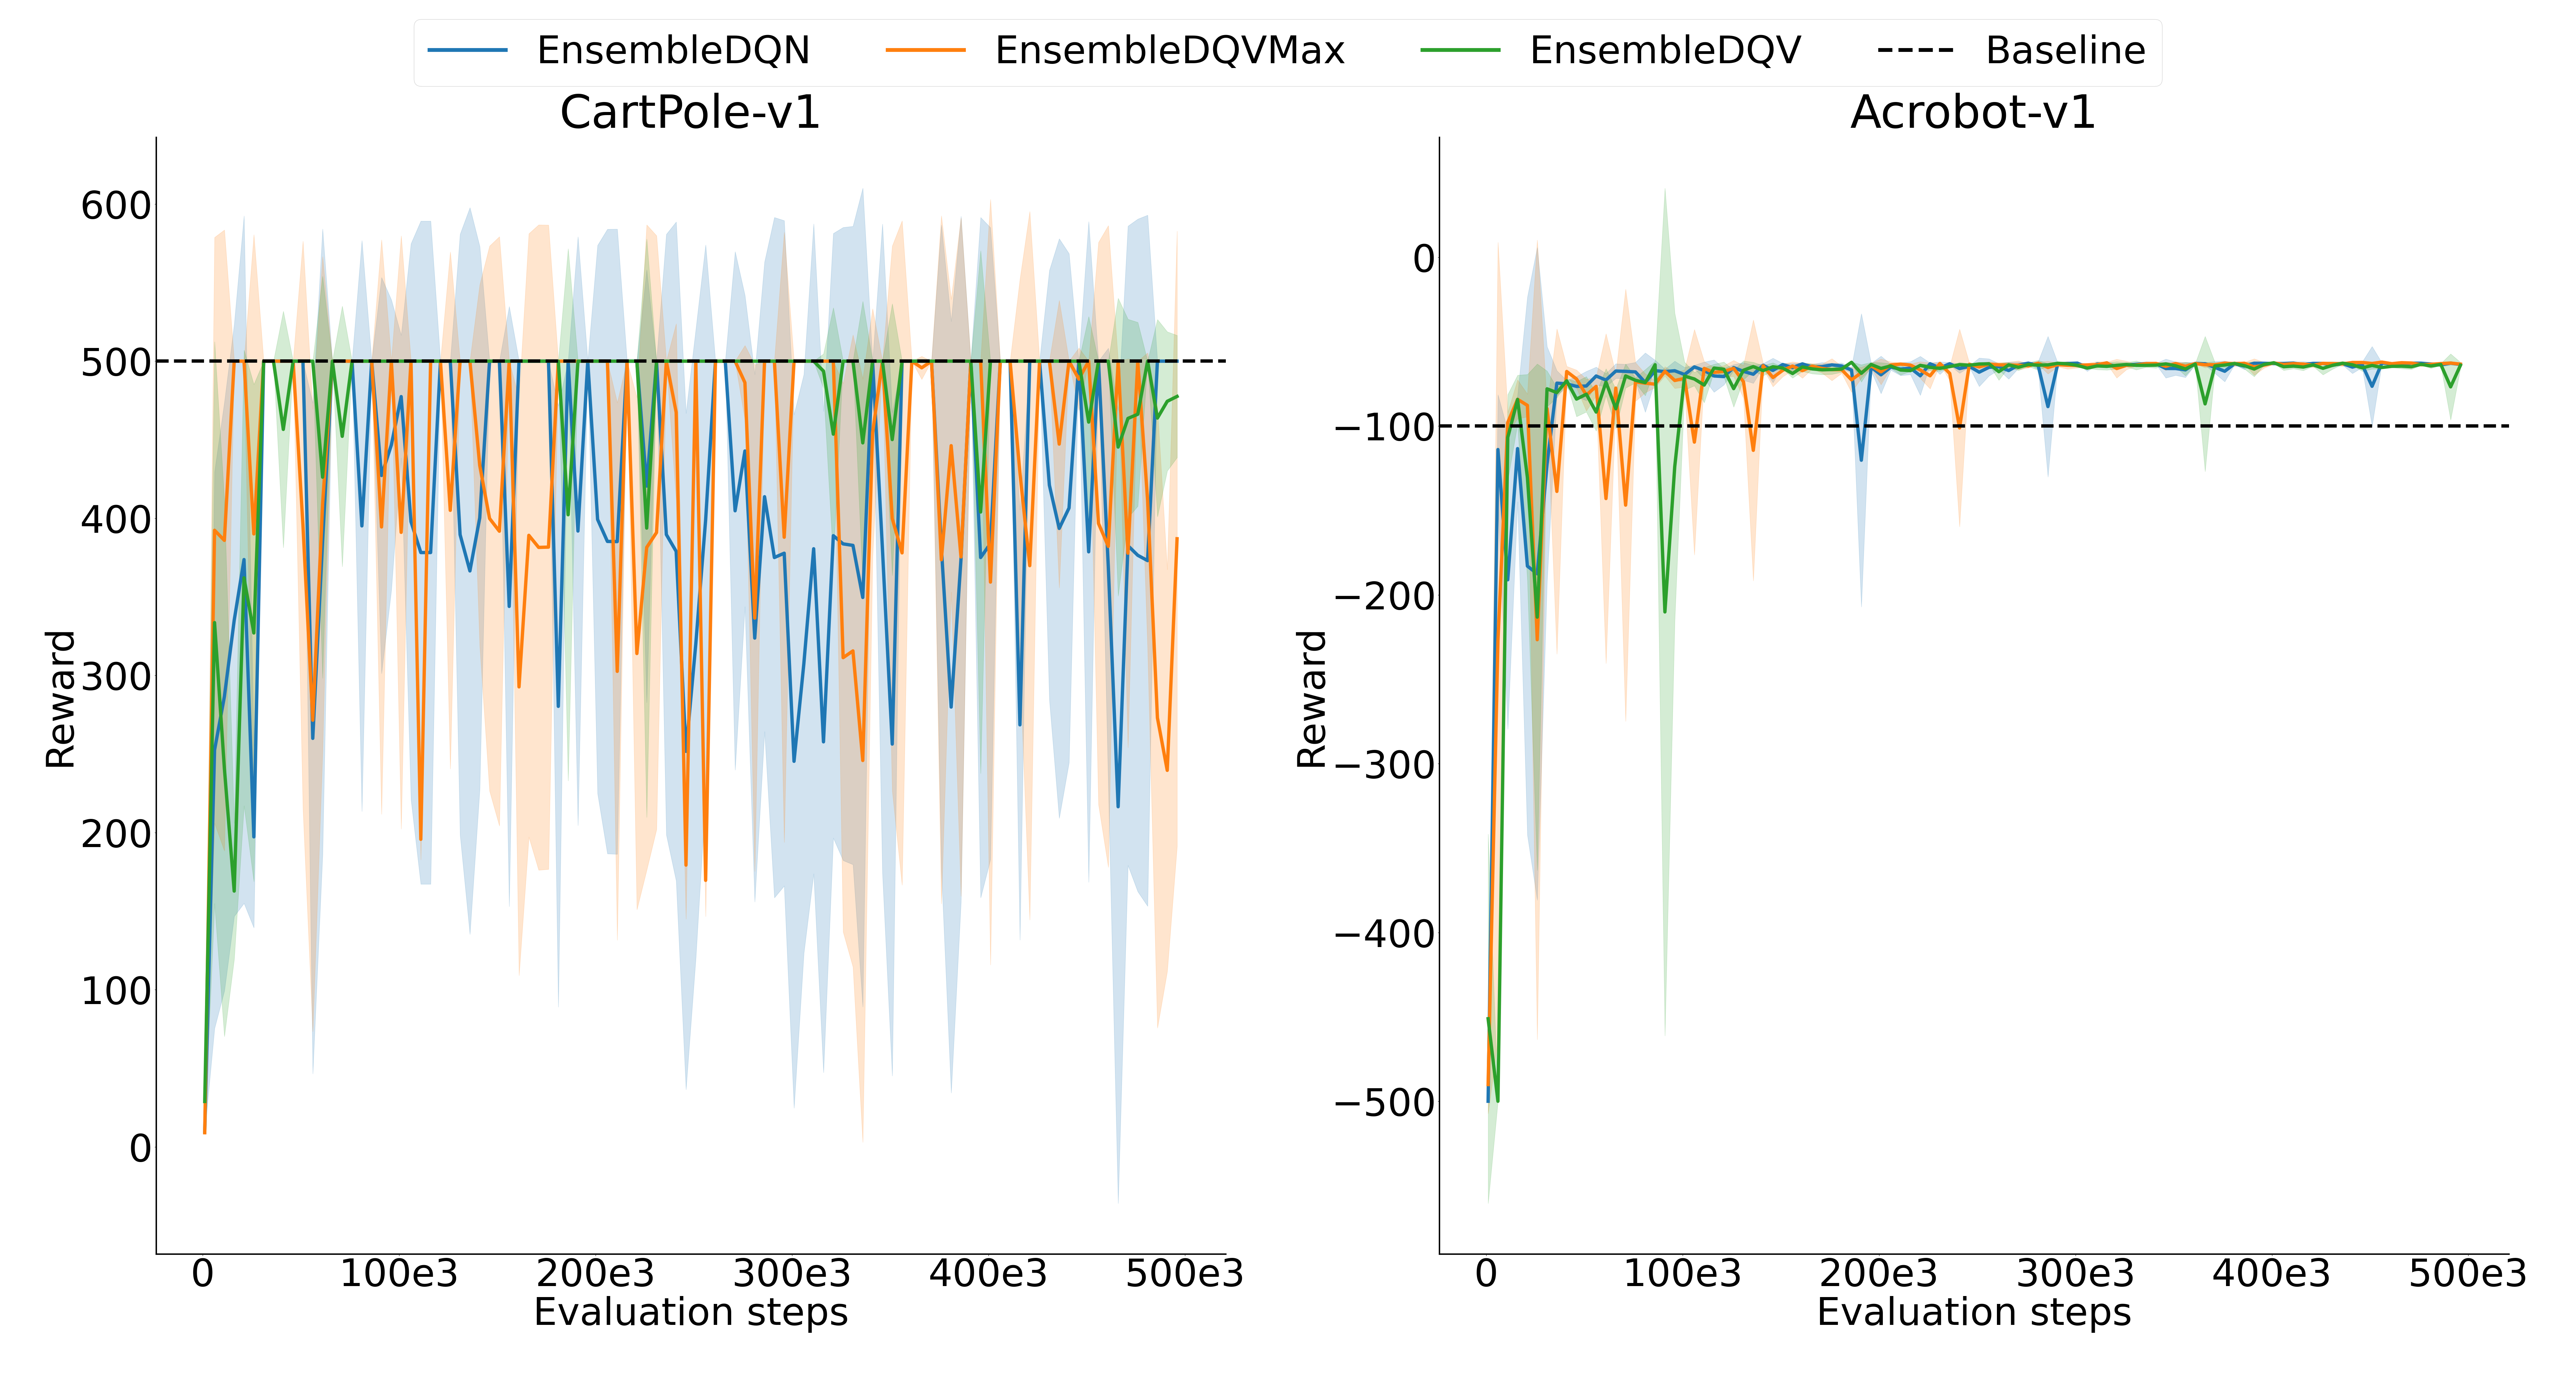
\includegraphics[width=.5\textwidth]{img/dshift_plots_ensembles_rwd.png}
  \caption{Ensemble agents reward signal}\label{fig:dshift_ensemble_rwd}
\end{figure}

\begin{figure}[H]
  \centering
  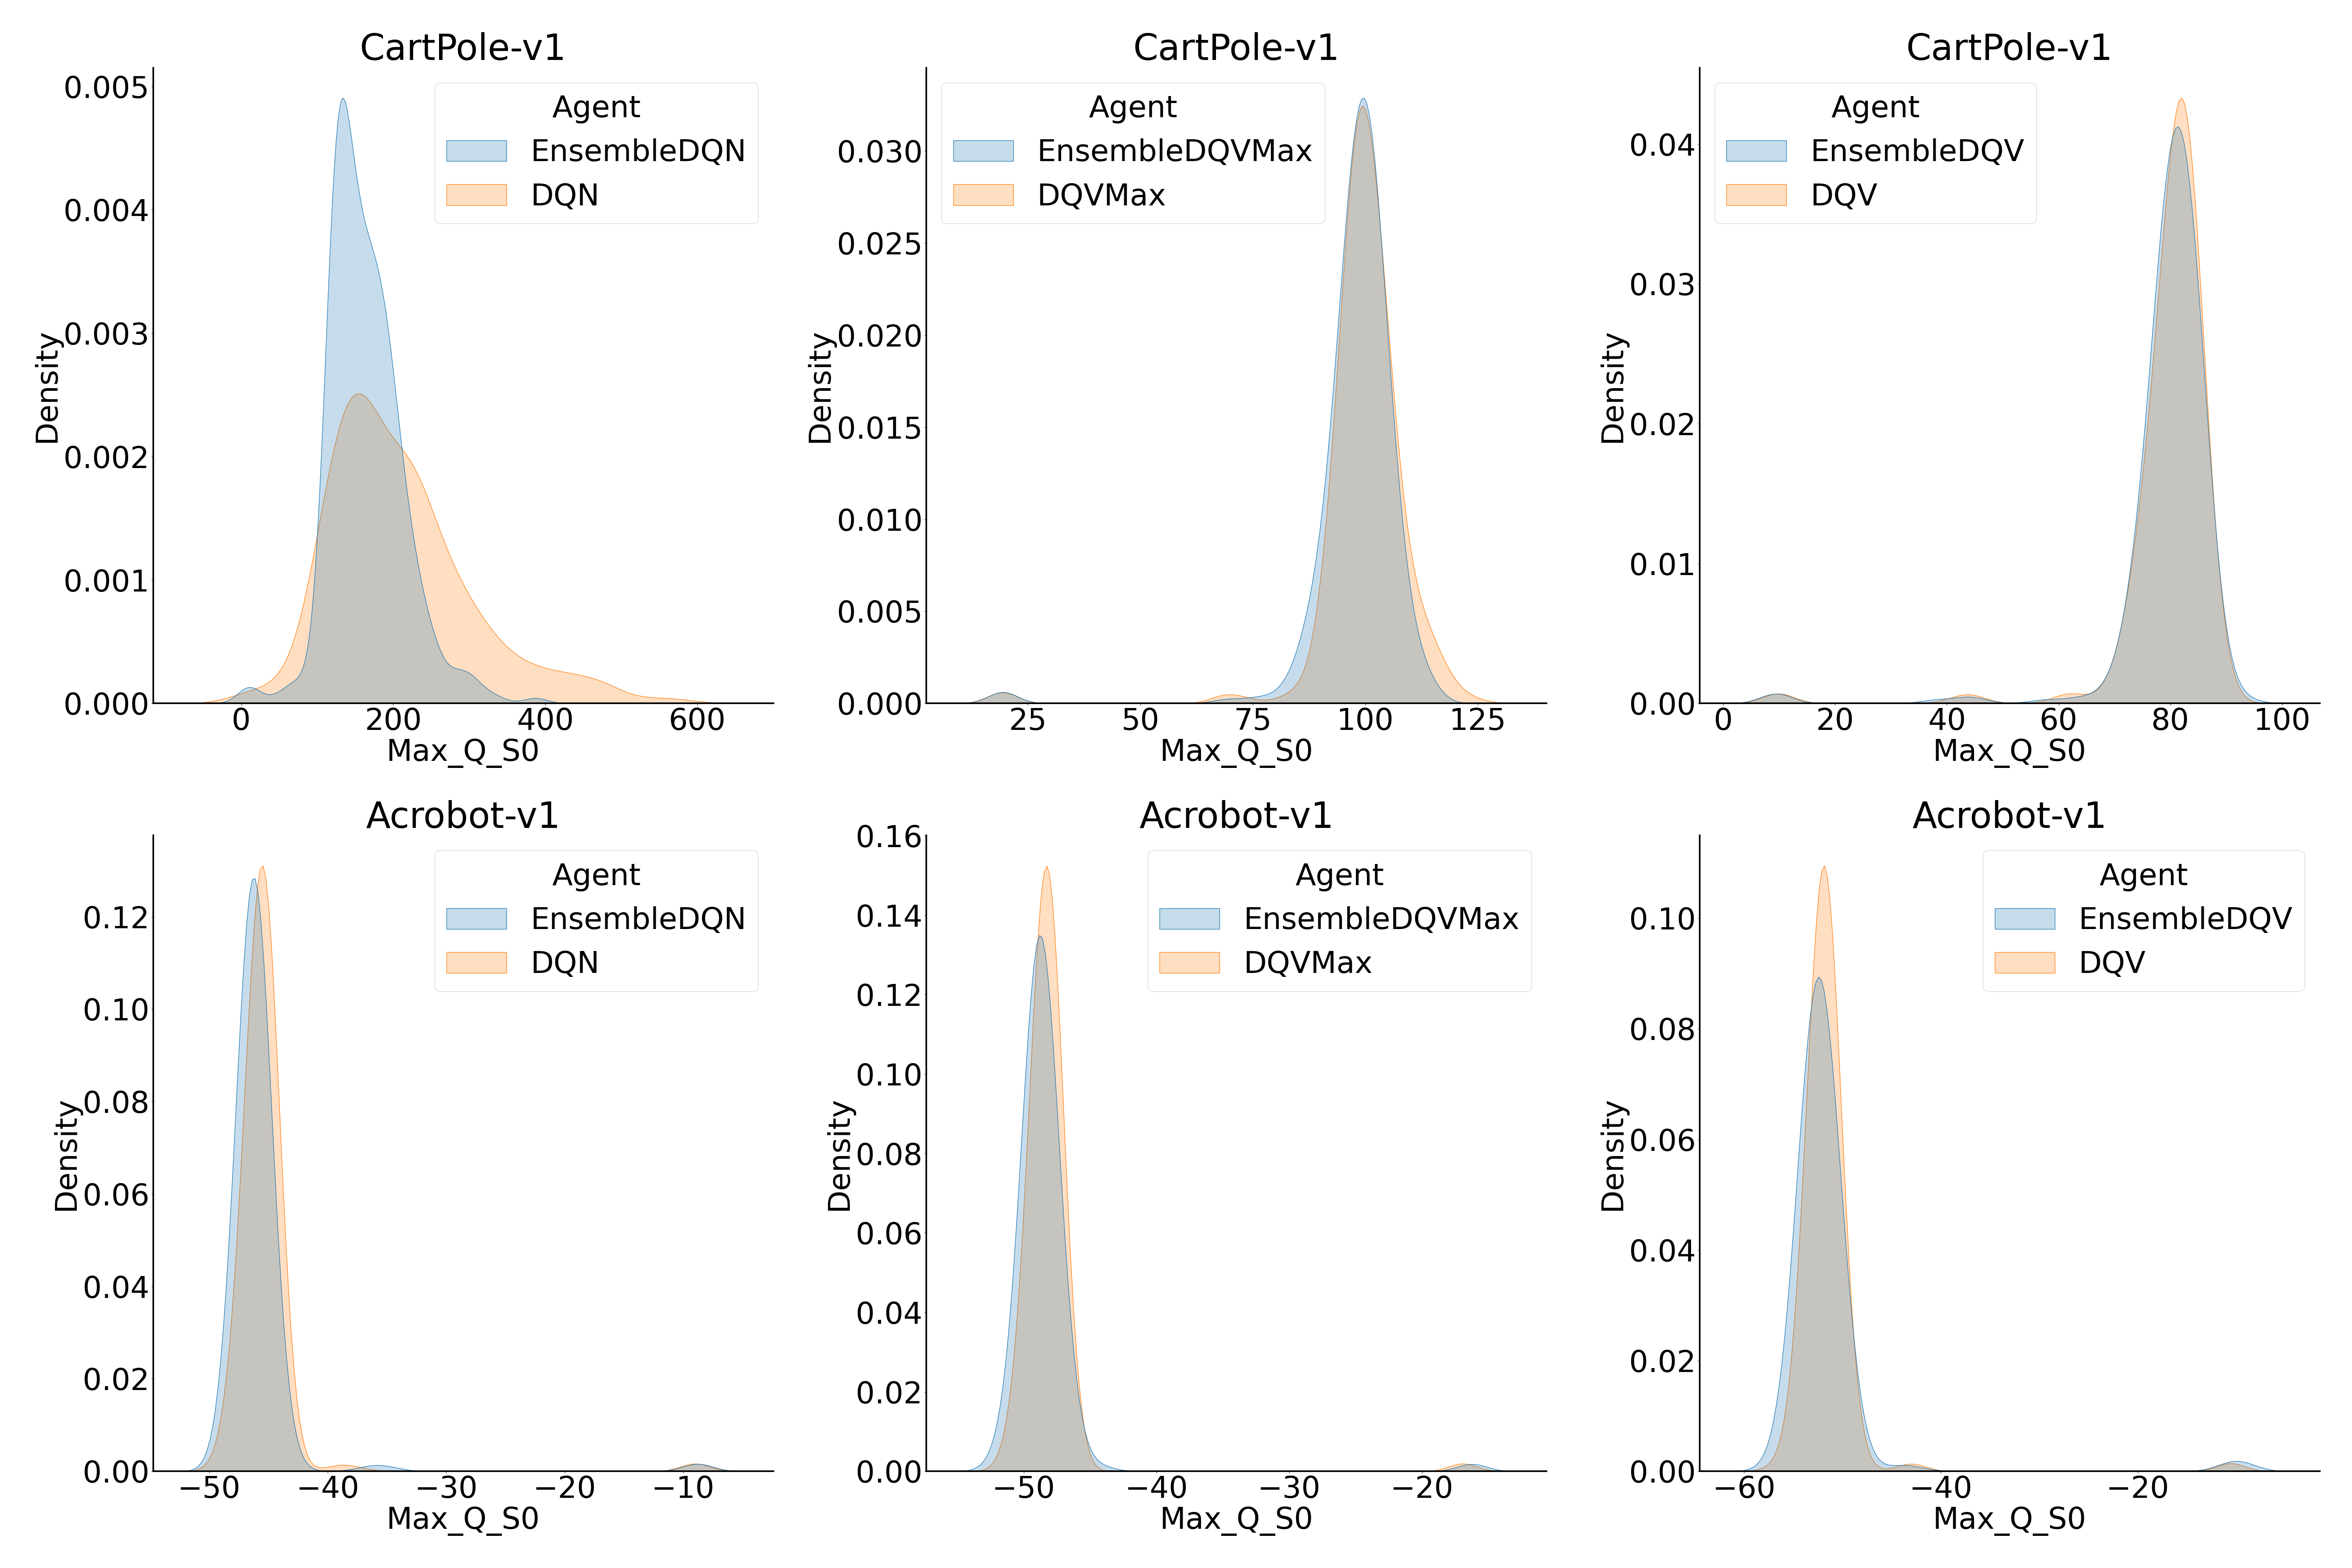
\includegraphics[width=.5\textwidth]{img/all_qv_dist.png}
  \caption{Distribution of maximum $Q$-values for $s_0$ for each agent
    and its ensemble variant}\label{fig:qv_dist}
\end{figure}

\begin{figure}[H]
  \centering
  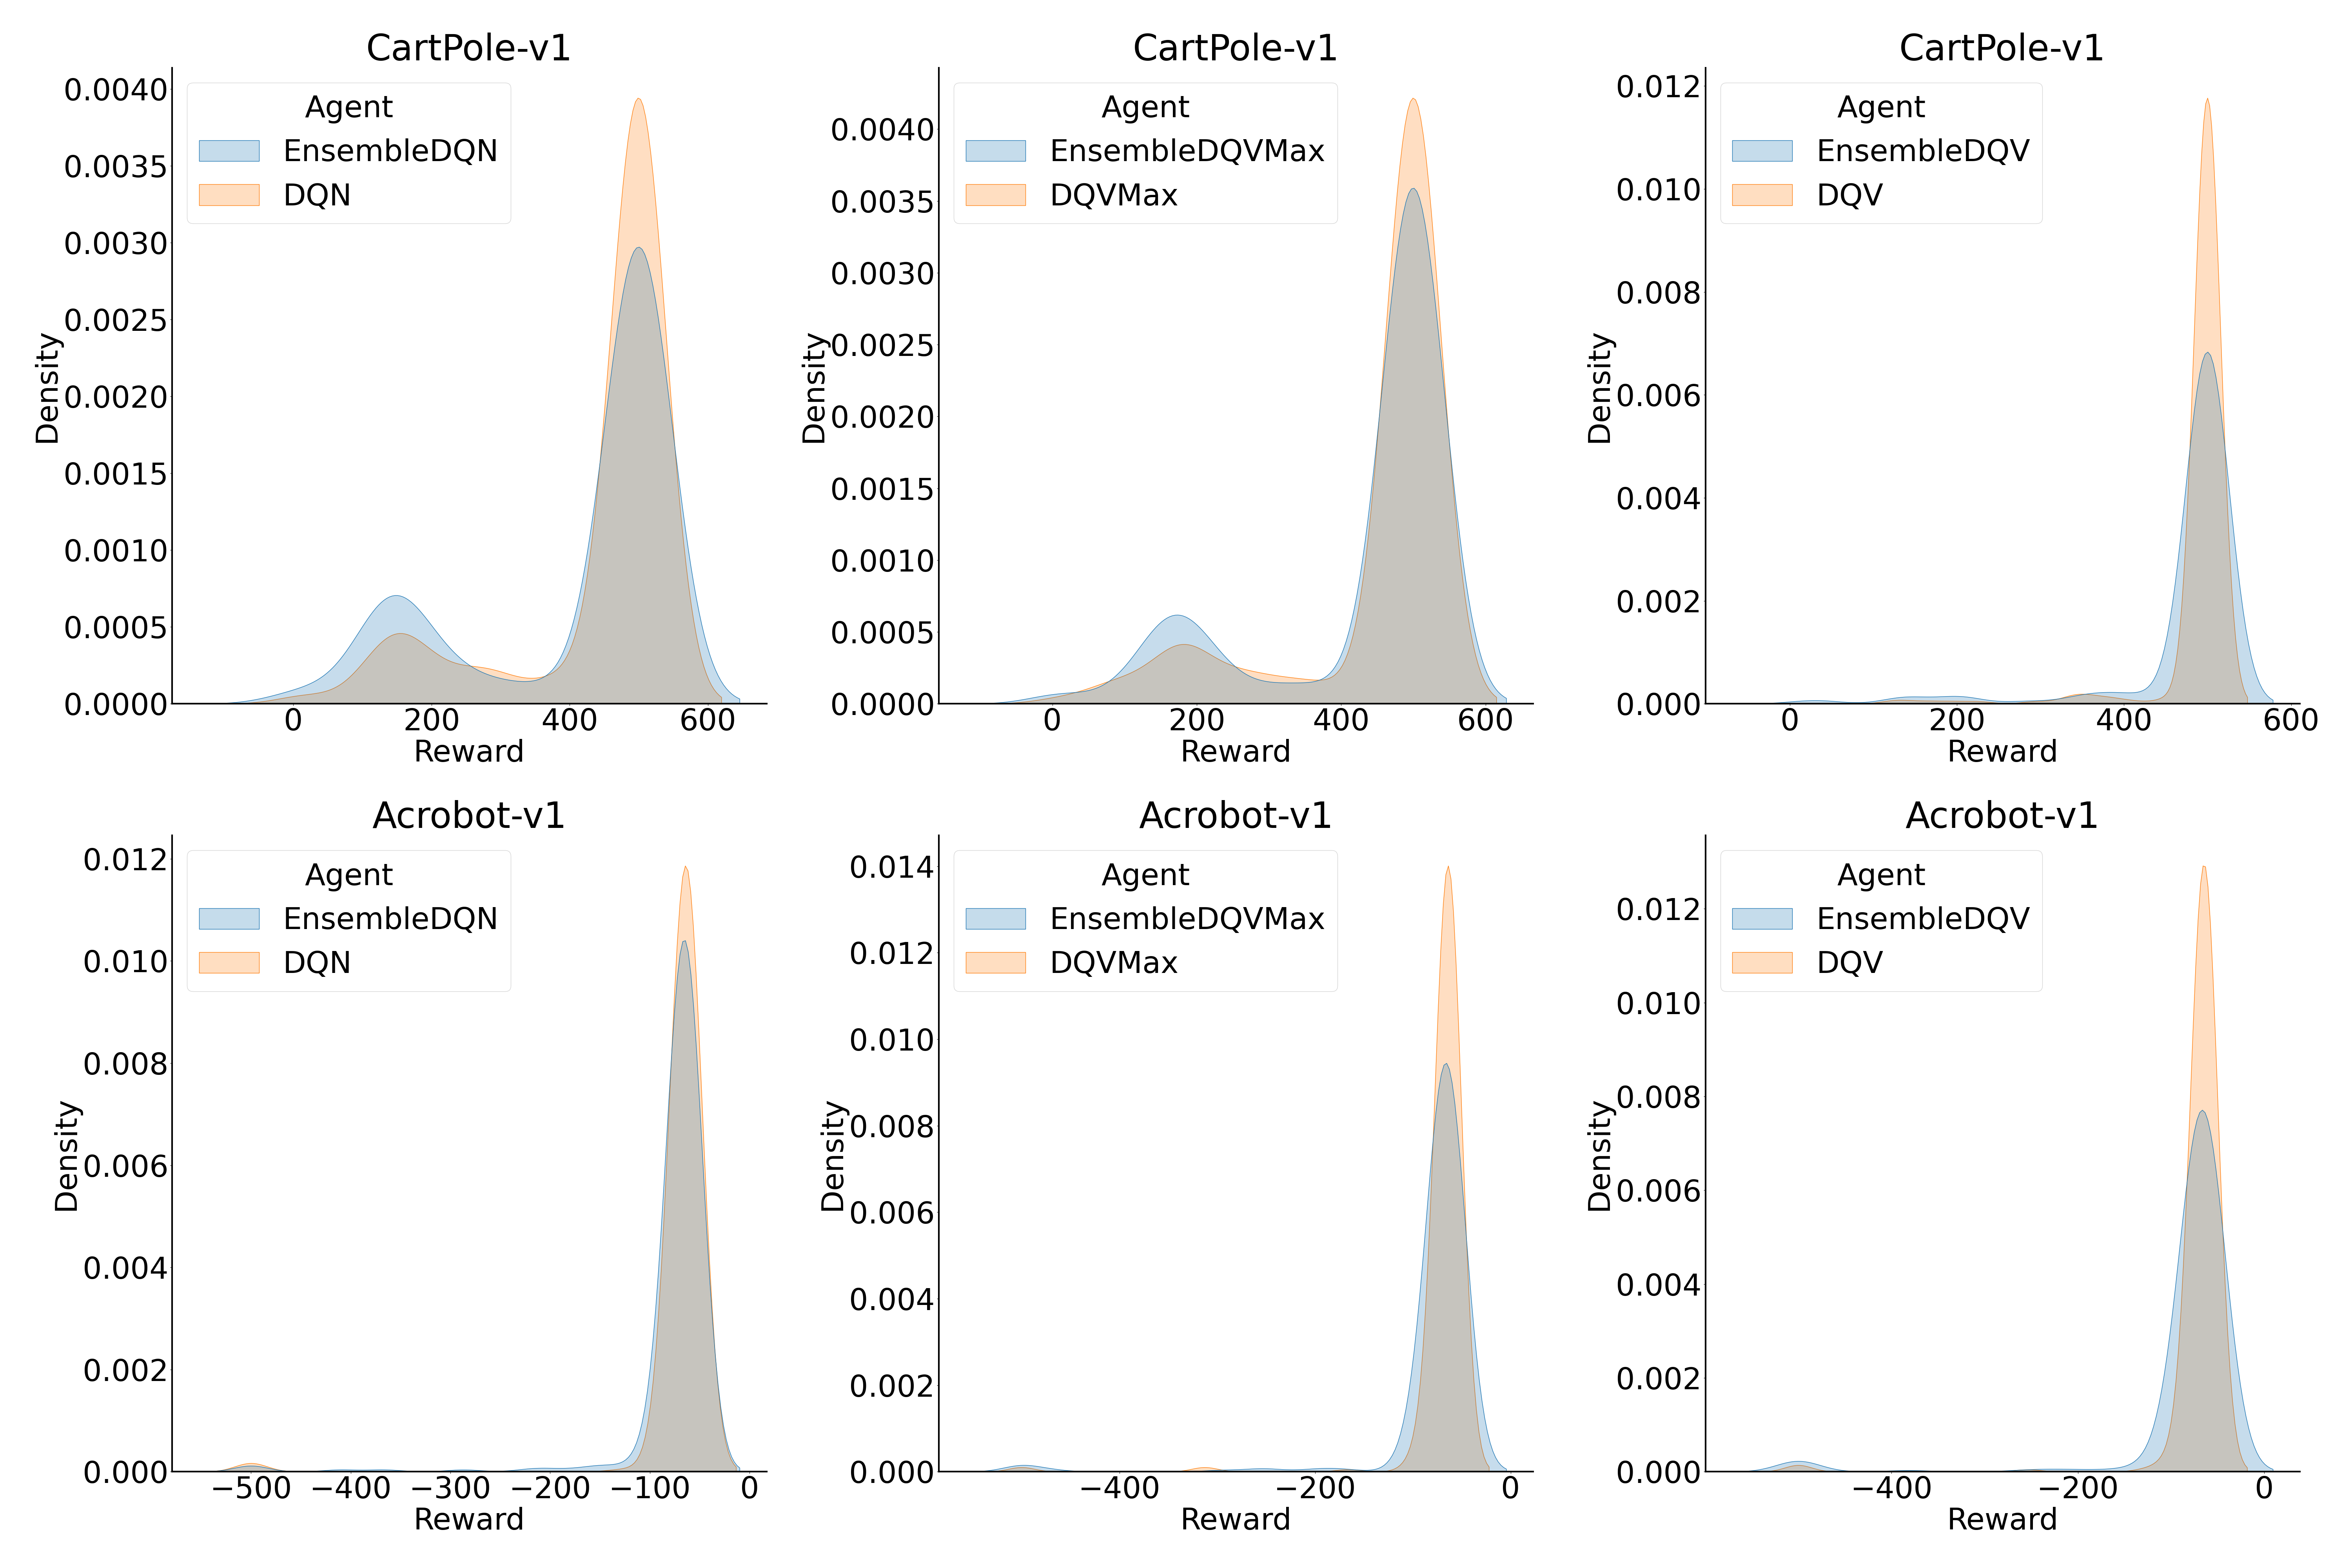
\includegraphics[width=.5\textwidth]{img/all_rwd_dist.png}
  \caption{Distribution of rewards for each agent and its ensemble
    variant}\label{fig:rwd_dist}
\end{figure}

\begin{figure}[H]
  \centering
  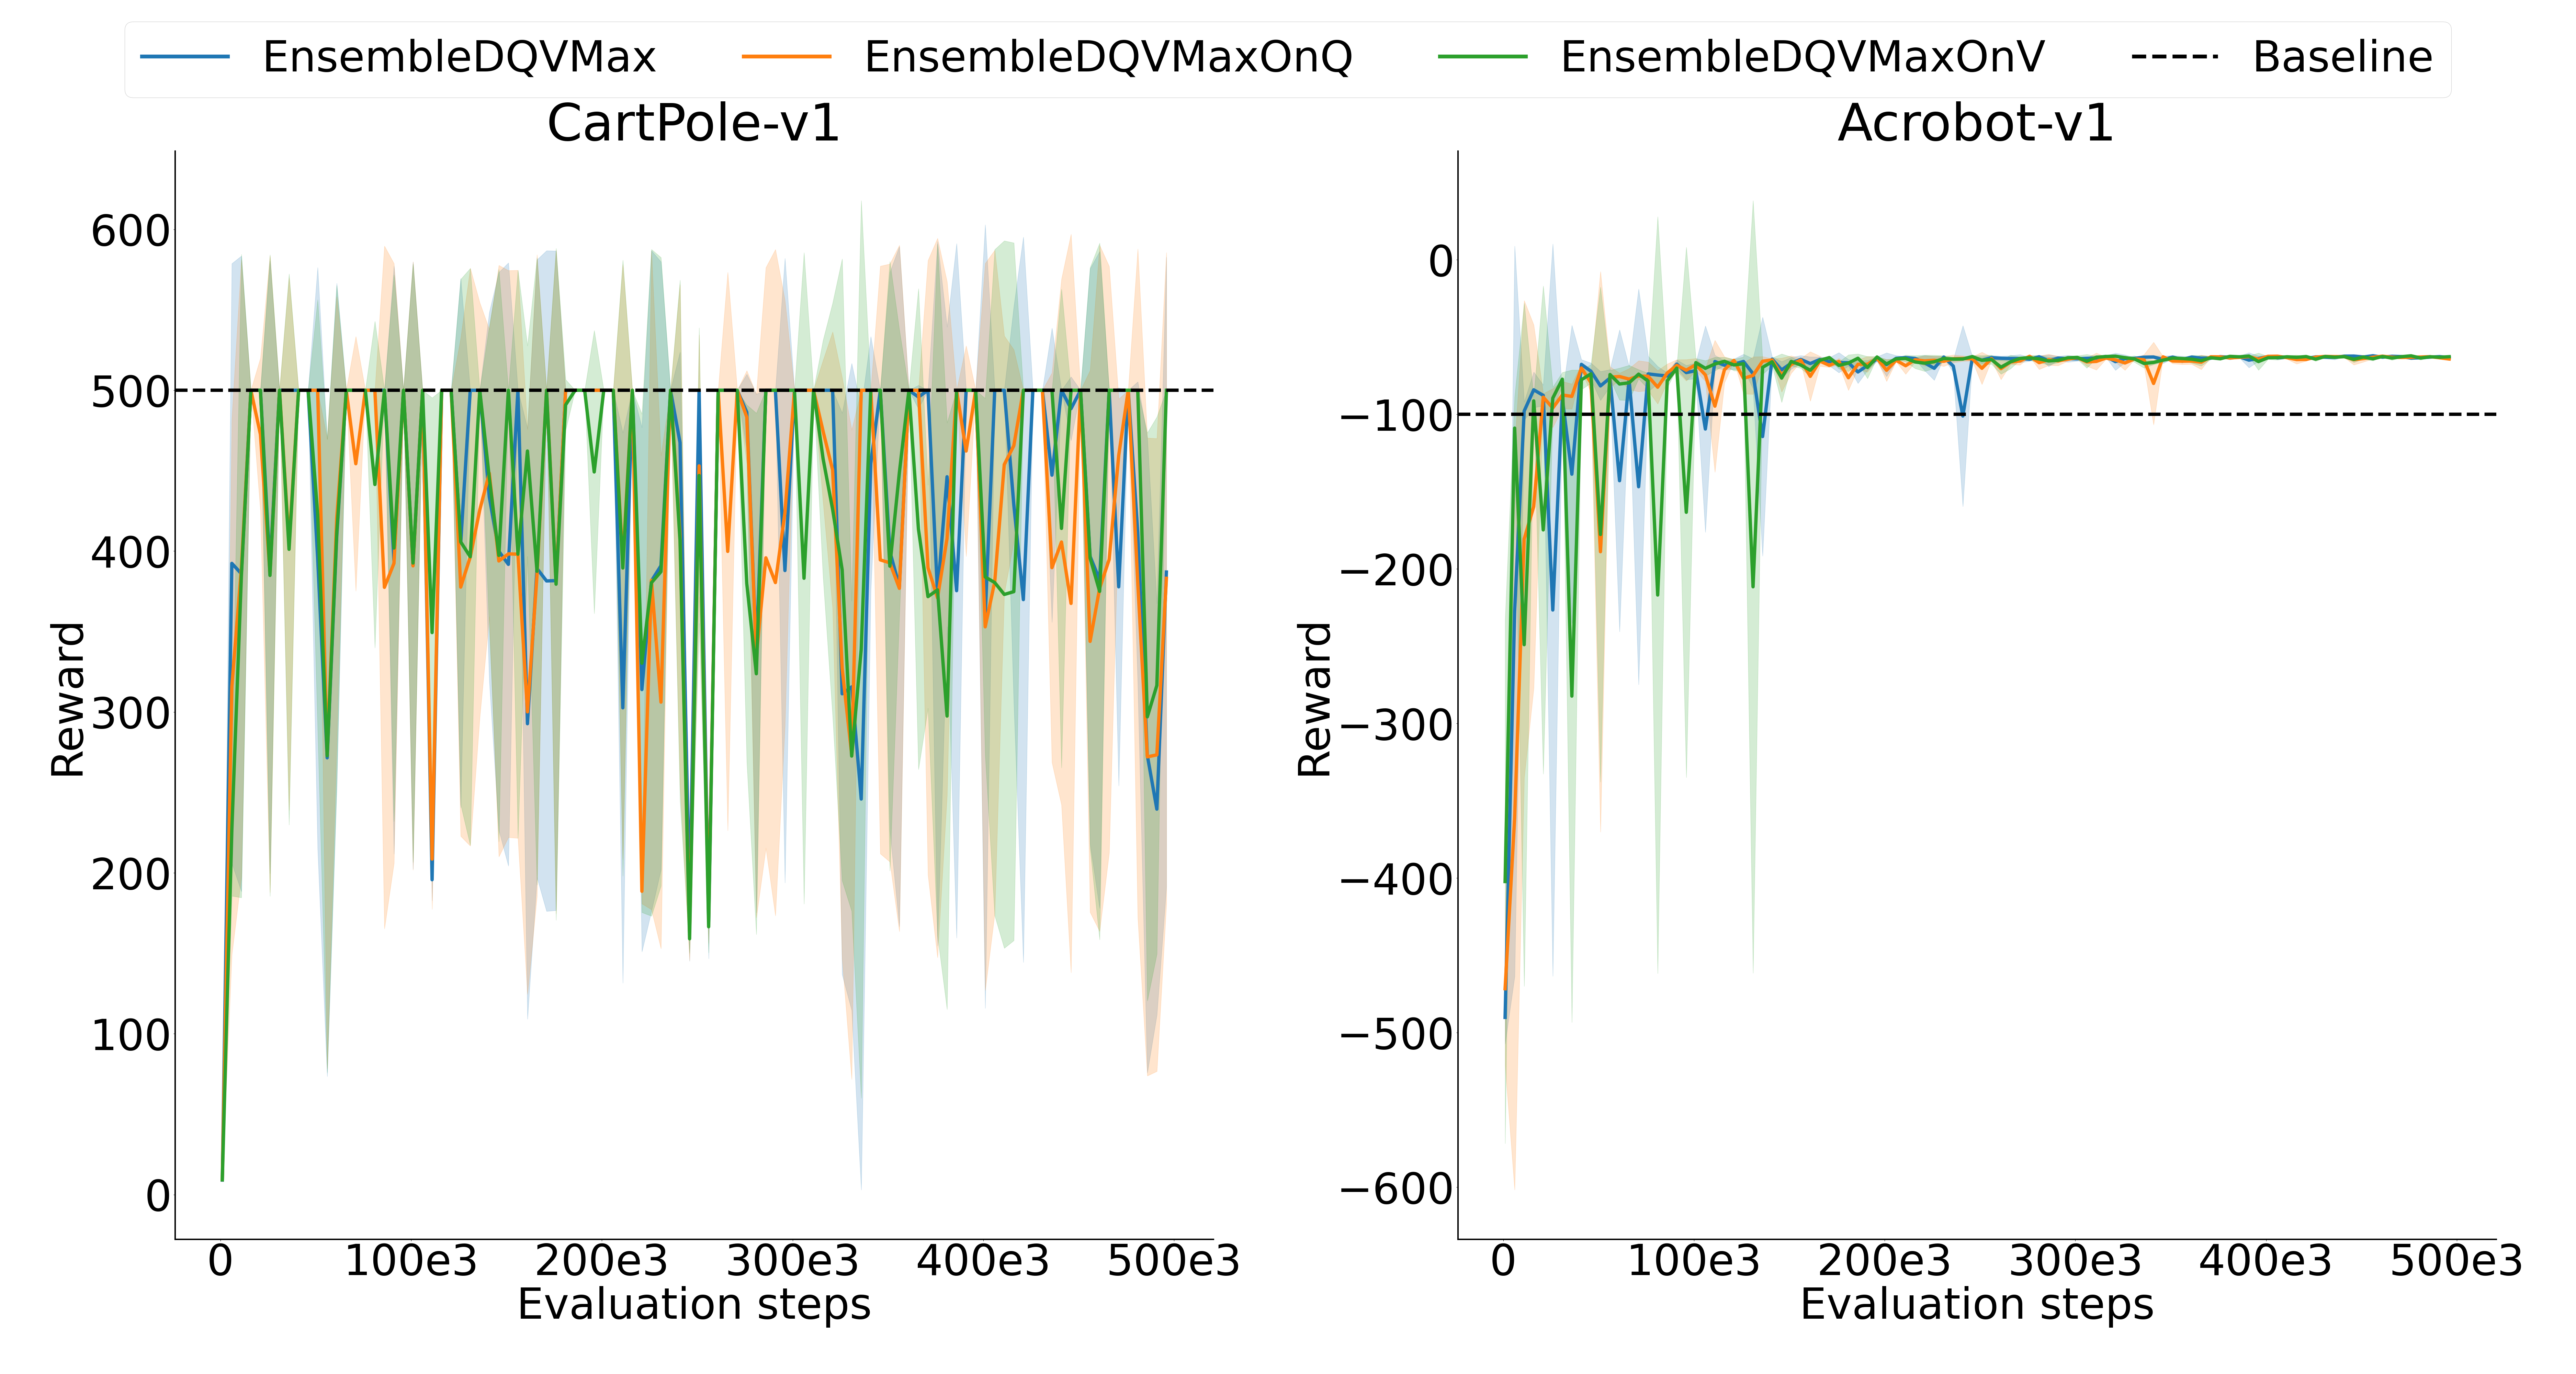
\includegraphics[width=.5\textwidth]{img/dshift_plots_ablation_rwd.png}
  \caption{Ensemble-DQV-Max reward signals for the ablations
    experiment}\label{fig:dshift_rwd_ablation}
\end{figure}

\begin{figure}[H]
  \centering
  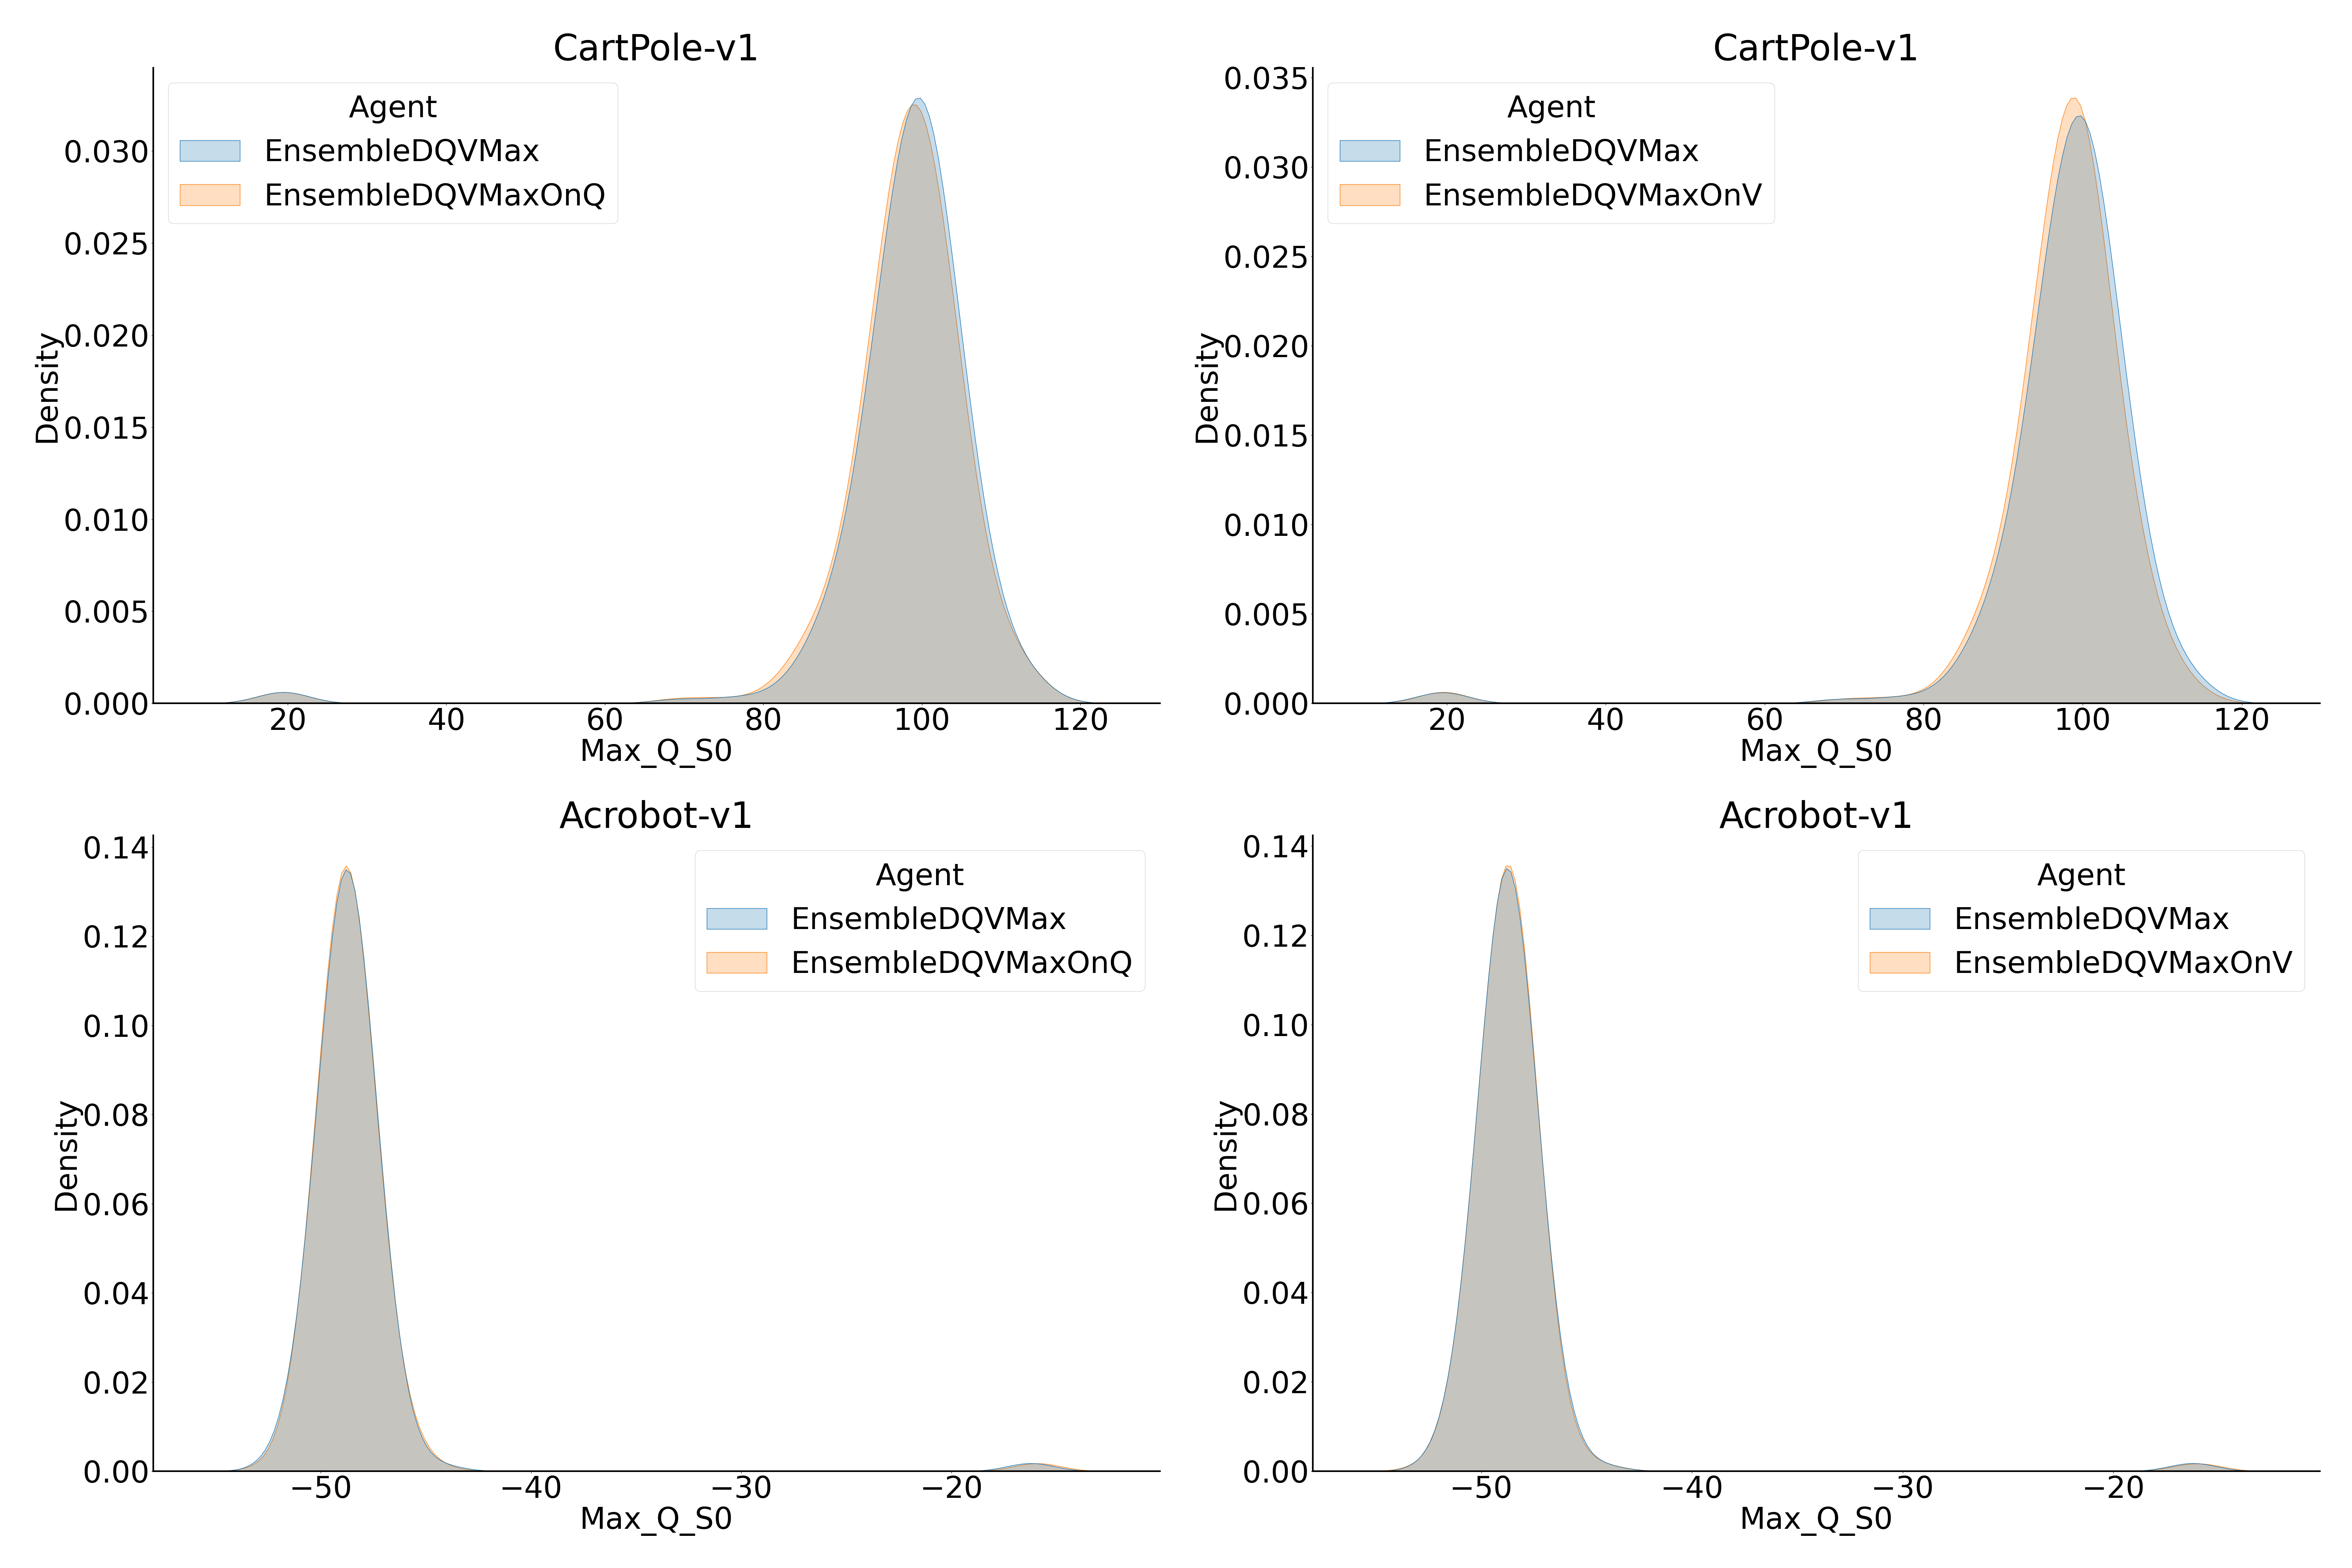
\includegraphics[width=.5\textwidth]{img/dqvmax_abl_qv_dist.png}
  \caption{Distribution of maximum $Q$-values for $s_0$ for
    Ensemble-DQV-Max and its ablations}\label{fig:dqvmax_abl_qv_dist}
\end{figure}

\begin{figure}[H]
  \centering
  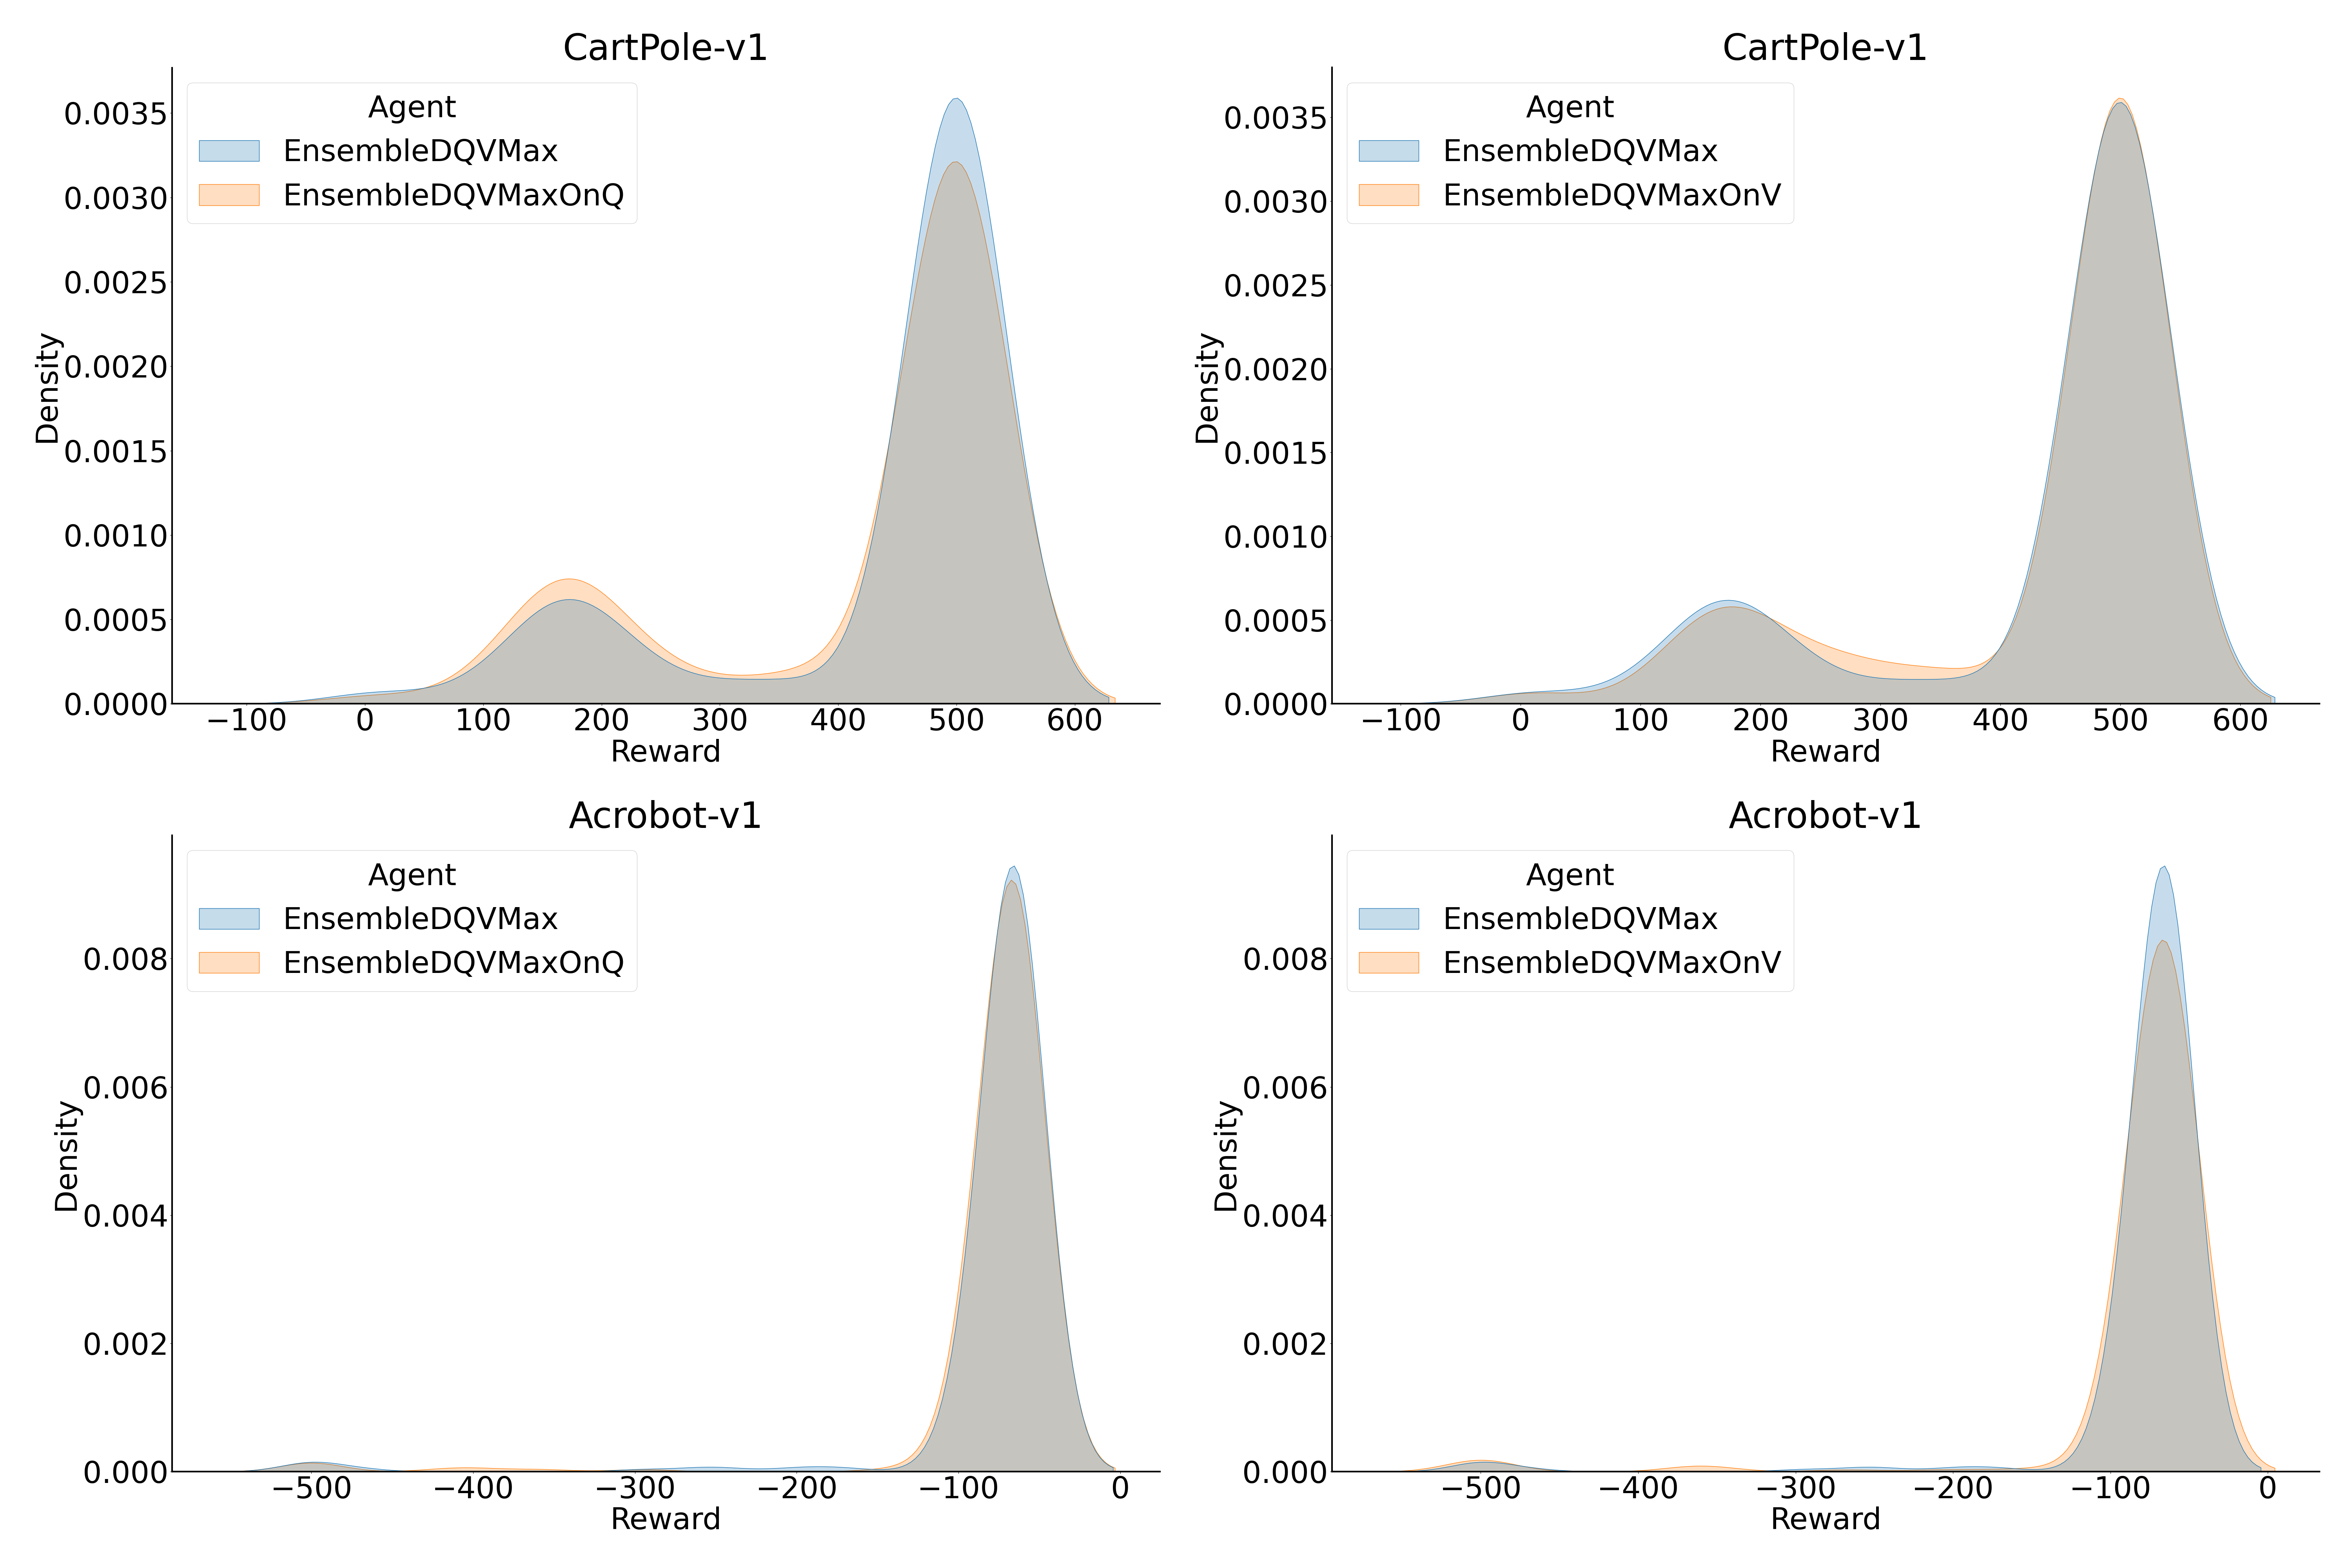
\includegraphics[width=.5\textwidth]{img/dqvmax_abl_rwd_dist.png}
  \caption{Distribution of rewards for Ensemble-DQV-Max and its
    ablations}\label{fig:dqvmax_abl_rwd_dist}
\end{figure}
